\textbf{\LARGE Scrum} \\ 

Scrum is an iterative and incremental development framework that coincides with the agile philosophy. It was first formalized by Ken Schwaber and Jeff Sutherland in 1995. The definition of Scrum; a framework within which people can address complex adaptive problems, while productively and creatively delivering products of the highest possible value\cite{Scrumguides}. \\

\textbf{\large Structure of Scrum}\\
The structure of Scrum is very different from traditional bottom-up approaches like the "Waterfall" model. In the "Waterfall" model, each project phase has a specific purpose and each phase is completed before preceding to the next. When all phases of a "Waterfall" project is completed, the product is completed. Scrum on the other hand, utilizes development cycles (called sprints), each development-cycle is usually between 2-4 weeks. A Scrum development cycle includes evaluation/prioritization, detailed requirements, design and analysis, implementation and developer testing, quality acceptance/acceptance testing. The framework incorporates all aspects of traditional development into one development cycle(See fig.1). The reason for this, is that the outcome of each development cycle may produce a potentially shippable feature or product. Thus, reducing time to market and increasing feedback. Increased frequency of feedback also makes Scrum more responsive and adaptable to changes.   

\begin{figure}[H]
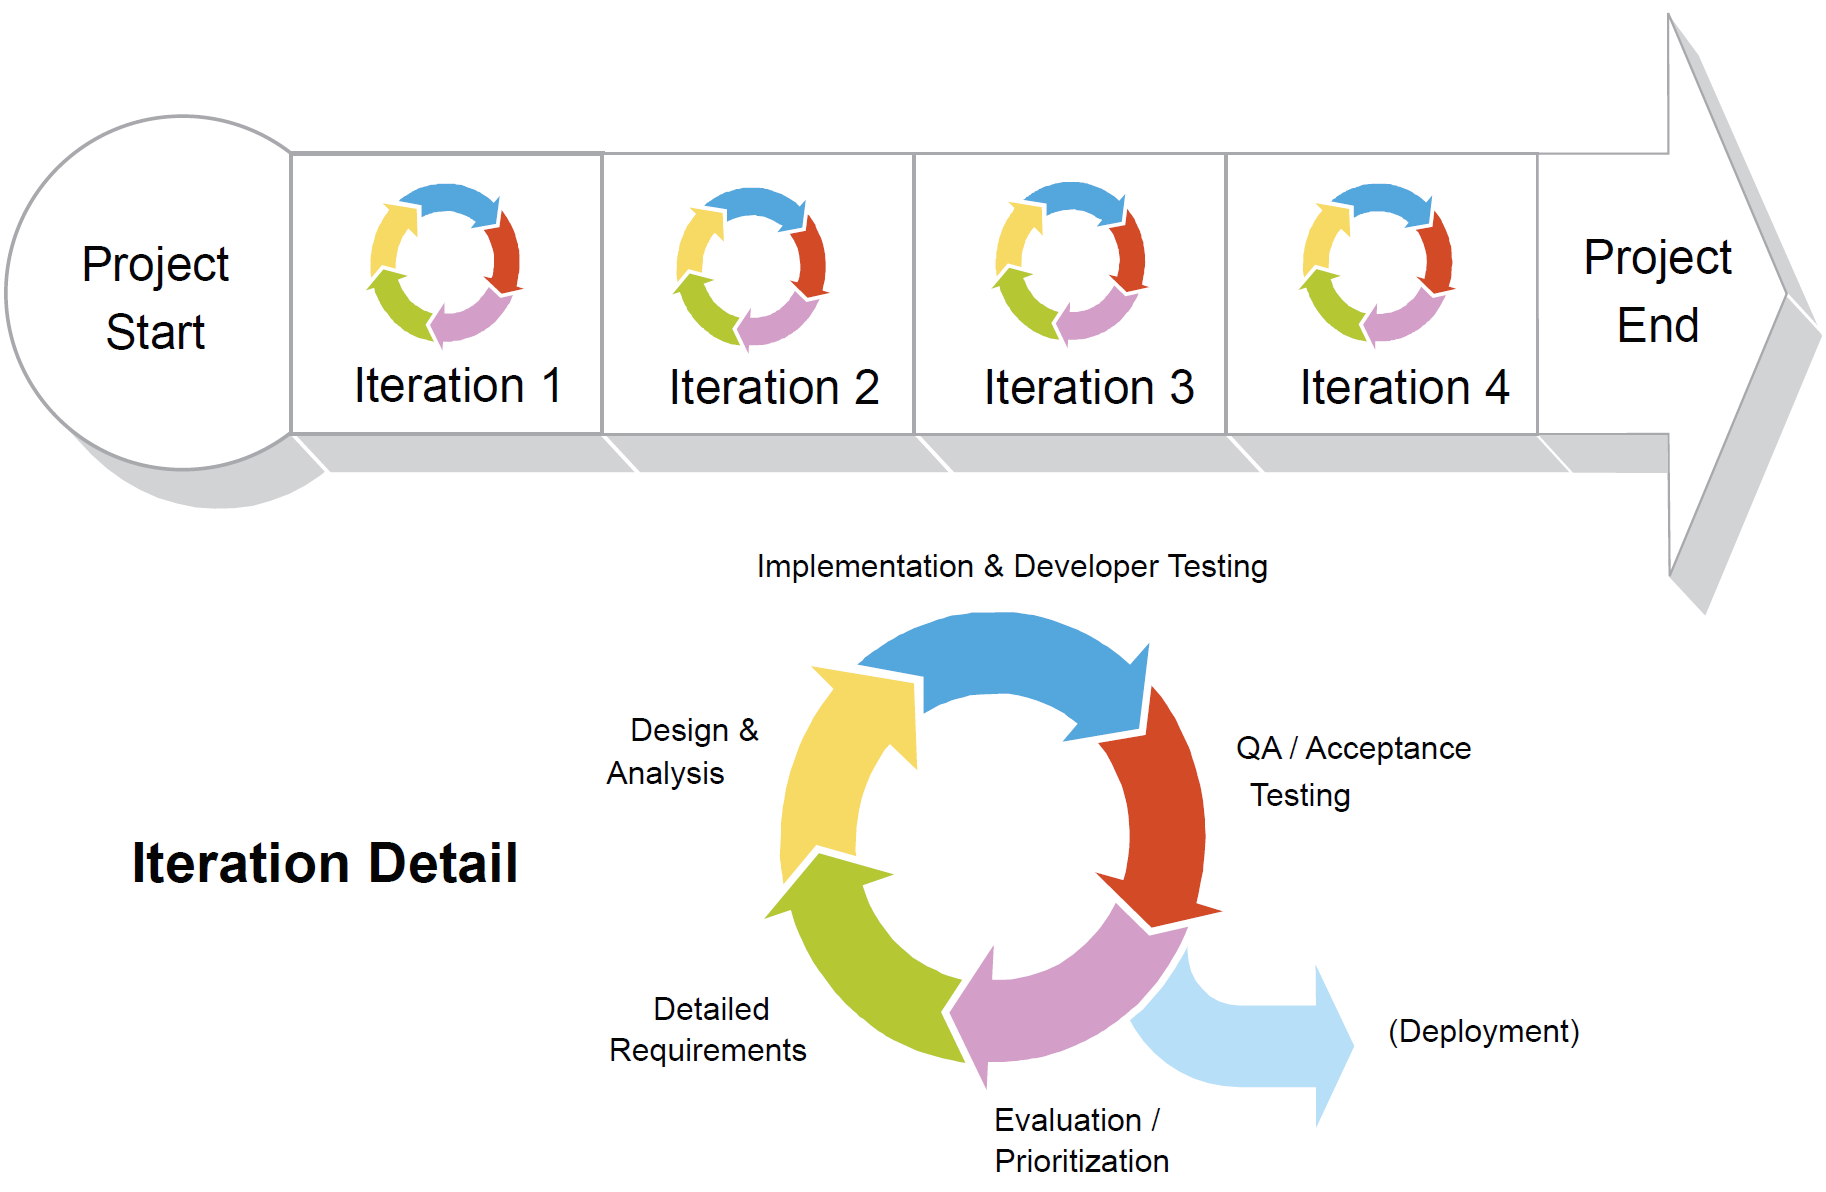
\includegraphics[scale=0.81]{VAPIQ-PICTURES/ScrumProcess.PNG}
 \caption*{Structure of Scrum}
\end{figure}

\clearpage 
\textbf{\LARGE Roles, Artifacts and Sprints} \\

The framework of Scrum is different from other agile models by specific concepts and practices, divided into the three categories of Roles, Artifacts, and Sprints (Development cycles). The roles in Scrum are; Product Owner, Scrum Master and Team Members. \\

The product owner has a leader-role with the responsibility of maximizing return on investment, the vision of the project, releases, prioritization of tasks and requirements (backlog items), and to preserve the wishes of the stakeholders. It is also the product owners job to determine if a project should be terminated or be continued.\\

The Scrum Master, is a facilitator with a leadership role, but has no management authority. He or she is a facilitator of Scrum and the team, ensuring the team understands the framework and that best practices are conducted. The Scrum Masters also shields the team from interferences and disturbances to make sure working conditions are optimal.\\

Last but not least, the team. The team often consists of people with different backgrounds and areas of expertise. Scrum requires that the team is self-organizing and gives them design space to execute the tasks in any way they see fit. The team works closely with each other and practice daily face- to- face communication in a ceremony often called "Daily Scrum". In this ceremony the team discuss what they have done, what they have to do and if anything is blocking them from making progress. The team plans the development- cycles (Sprints) in close cooperation with the Product Owner, one sprint at the time. \\

The Artifacts of Scrum is the Backlog, Sprint Backlog and Burn Down Chart. The Backlog specifies what to do based on the customers wishes, most often formulated as user stories (As a.., i want.., because/why..). These user stories are then prioritized in the backlog.\\

Backlog items are selected to go into the sprint backlog, and are then broken down by the team into tasks. Tasks are sorted as "to do", "in progress" and "done". The team are free to take on the tasks they see fit and can manage. As a general rule, one task should never exceed 3 days and should preferably be less than one days work. If tasks are bigger than this, they should be broken into smaller more manageable pieces.\\

The last artifact is the burn down chart, this chart is a measure of time remaining work for the whole team. As user stories and tasks are generated, they are often allocated story points. Story points is the relative measure of the amount of estimated work in a user story or task. The scaling of the story points does not have a standard, but are decided by the team themselves.


\newpage
\textbf{\LARGE Scrum Ceremonies} \\
\begin{wrapfigure}{l}{0.5\textwidth}
  \begin{center}
    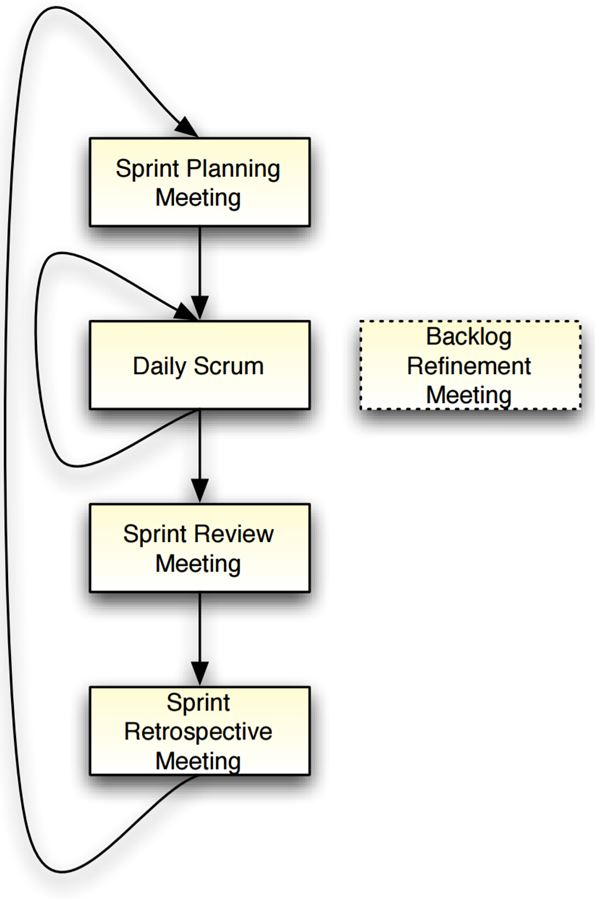
\includegraphics[scale=0.4]{VAPIQ-PICTURES/ScrumActivities}
  \end{center}
  \caption*{Scrum Activities}
\end{wrapfigure}
In Scrum, meetings are refereed to as ceremonies. The different ceremonies are; sprint planning meeting, daily Scrum, sprint review meeting, sprint retrospective meeting and backlog refinement meeting(See fig.2). \\

In a sprint planning meeting the attendees are; Scrum Master, Product Owner and Scrum Team. This meeting clarifies what tasks has to be completed in order to achieve the sprint goals and what is required in 
the user stories. The input for this ceremony is a Backlog prioritized by the Product Owner. In this meeting, stories are given a relative time estimate called story points and stories are divided into tasks. The output of this activity is the sprint backlog and sprint goal.\\

Daily Scrum is performed by the whole team once every day, the purpose of this meeting is to inform the team on progress and to promote discussion. The meeting is no more than 15 minutes. Each team member presents; what they've done, what they are going to do, and what is blocking them from making progress. This also means the team can adapt during the sprint.\\

Sprint review, also called sprint demo meeting and is held at the end of each sprint. This is where the outcome (product increment) of the sprint is presented to the product owner, team and stakeholders. The outcome is evaluated and feedback is given. The feedback from this meeting may result in new requirements in the Product Backlog, and a new prioritization of existing Product Items.\\

In the sprint retrospective meeting, the last sprint is reviewed. Team members discuss; what worked, what did not work, are our estimates right, have we over committed to work, etc. The purpose is to evaluate the process of the last sprint and learn from success and mistakes. The review gives insight into how the next sprint should be planned and executed, hopefully making it a more efficient sprint than the last.\\

Backlog refinement, often called grooming is not part of the main loop but is an important activity. This activity has as purpose to further refine the elements in the backlog. The whole team attends the meeting.



\newpage
\textbf{\LARGE What is agile?} \\

The term agile first appeared in the "Manifesto for Agile Software Development"\cite{agileManifesto}. The manifest was written by 17 representatives with different backgrounds within software and systems engineering in 2001. The goal of this manifest was to develop an alternative approach to the traditional documentation driven development process.
\\

The founders saw a need for a more adaptive model, based on other values and principles than heavy process and documentation. This was the birth of agile, 4 values and 12 principles formulated in the "agile manifesto". 


% Values and Principles
\begin{figure}[h]
     \begin{minipage}[t]{0.3\textwidth}
    \textbf{Values:}
        \begin{itemize}
            \item Individuals and interactions over processes and tools
            \item Working features over comprehensive documentation
            \item Customer collaboration over contract negotiation
            \item Responding to change over following a plan
        \end{itemize}
     \end{minipage}
        \hfill
    \begin{minipage}[t]{0.3\textwidth}
        \textbf{Principles:}
        \begin{itemize}
            \item Our highest priority is to satisfy the customer
                  through early and continuous delivery
                  of valuable software.
            \item Welcome changing requirements, even late in 
                    development. Agile processes harness change for 
                    the customer's competitive advantage.
            \item Deliver working software frequently, from a 
                    couple of weeks to a couple of months, with a 
                 preference to the shorter timescale.
            \item Business people and developers must work 
                    together daily throughout the project.
            \item Build projects around motivated individuals. 
                Give them the environment and support they need, 
                and trust them to get the job done.
            \item  Working software is the primary measure of progress.
        \end{itemize}
    \end{minipage}
            \hfill
    \begin{minipage}[t]{0.3\textwidth}
    \textbf{}
        \begin{itemize}
            \item The most efficient and effective method of 
                conveying information to and within a development 
                team is face-to-face conversation.
            \item Agile processes promote sustainable development. 
                    The sponsors, developers, and users should be able 
                 to maintain a constant pace indefinitely.
            \item Continuous attention to technical excellence 
                    and good design enhances agility.
            \item Simplicity--the art of maximizing the amount 
                    of work not done--is essential.
            \item The best architectures, requirements, and designs 
                    emerge from self-organizing teams.
            \item At regular intervals, the team reflects on how 
               to become more effective, then tunes and adjusts 
               its behavior accordingly.
        \end{itemize}
    \end{minipage}
\end{figure}


\newpage

The manifest marks a paradigm change in the way many development processes are conducted. 
In traditional development models, like the "Waterfall" approach, the development team must have a rigorous understanding of the stakeholders needs and they have to get requirements right on the first try. Extensive and time consuming planning is done up front and all the project phases are performed in an evolutionary fashion. The term evolutionary, means that project phase do not overlap and that one phase is completed before the next can begin.  
\\
The problem with this approach is that much work is done before getting feedback and no features are produced until late in the project. Customers are often held at a distance under development, and do not see the product until the unveiling of a prototype. Reviews are performed after each phase to determine if the project is on the right track or not, but testing is performed only after the system integration phase. 
\begin{figure} [H]
 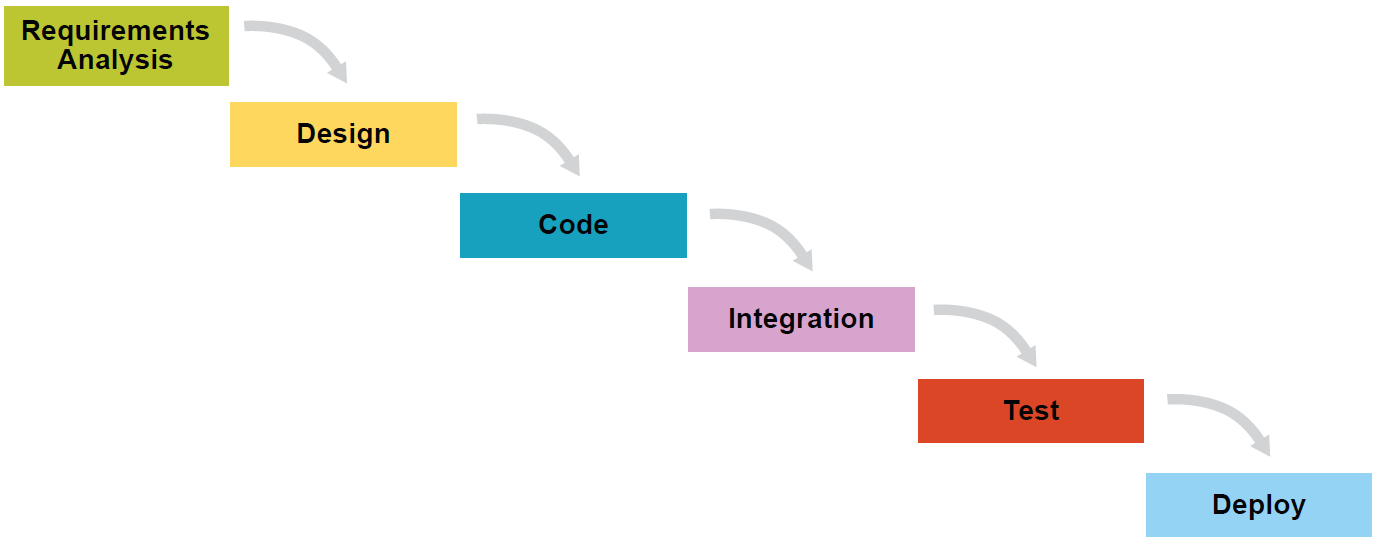
\includegraphics{VAPIQ-PICTURES/WaterFall.PNG}
 \caption*{Waterfall Model}
\end{figure} 

The test phase is typically where many problems are unveiled. And if they are, all work done prior to this phase must be revised to accommodate the necessary changes. The lack of customer interaction as the project progresses may result in the project taking another direction than what the customer originally wanted. Thus, this approach does not handle changes well and can be time consuming. It may contribute to unnecessary amounts of risk, uncertainty, cost and may result in the customer getting the wrong product.\\ 

The disadvantages of the traditional engineering approach, inspired the definition of agile.
The goal is to increase customer satisfaction and reduce delivery times while promoting creativity, motivation and quality. 






